\section{Introduction}

Convolutional Neural Networks (CNN) is one of the most if not the most popular neural network models for computer vision. They utilize a kernel for recognizing patterns within images. CNNs make use of the locality aspect of objects within images because of the kernel; instead of considering each and every pixel in the image, the kernel is able to take only a subset of that image and share weights or network parameters at many locations. Because of this, CNNs lead the way for image recognition in deep learning. 

In this lab exercise, CNNs must be utilized to detect hair types. There are three main types to classify: curly, straight, and wavy hair. Figure \ref{fig:hairtypes} shows an example from each hair type.

\begin{figure}[H]
  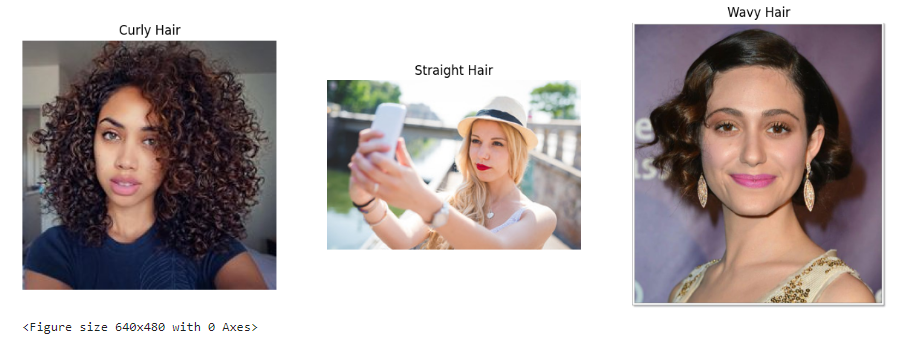
\includegraphics[width=\linewidth]{figures/hairtypes.png}
  \caption{Hair Types Example}
  \label{fig:hairtypes}
\end{figure}
